% ------------------------------------------------------------------
\chapter{Computational blocks}\label{s:blocks}
% ------------------------------------------------------------------

This chapters describes the individual computational blocks supported by \matconvnet. The interface of a CNN computational block !<block>! is designed after the discussion in \autoref{s:fundamentals}. The block is implemented as a MATLAB function !y = vl_nn<block>(x,w)! that takes as input MATLAB arrays !x! and !w! representing the input data and parameters and returns an array !y! as output. In general, !x! and !y! are 4D real arrays packing $N$ maps or images, as discussed above, whereas !w! may have an arbitrary shape.

The function implementing each block is capable of working in the backward direction as well, in order to compute derivatives. This is done by passing a third optional argument !dzdy! representing the derivative of the output of the network with respect to $\by$; in this case, the function returns the derivatives ![dzdx,dzdw] = vl_nn<block>(x,w,dzdy)! with respect to the input data and parameters. The arrays !dzdx!, !dzdy! and !dzdw! have the same dimensions of !x!, !y! and !w! respectively (see \autoref{s:back}).

Different functions may use a slightly different syntax, as needed: many functions can take additional optional arguments, specified as a property-value pairs; some do not have parameters  !w! (e.g. a rectified linear unit); others can take multiple inputs and parameters, in which case there may be more than one !x!, !w!, !dzdx!, !dzdy! or !dzdw!. See the rest of the chapter and MATLAB inline help for details on the syntax.\footnote{Other parts of the library will wrap these functions into objects with a perfectly uniform interface; however, the low-level functions aim at providing a straightforward and obvious interface even if this means differing slightly from block to block.}

The rest of the chapter describes the blocks implemented in \matconvnet, with a particular focus on their analytical definition. Refer instead to MATLAB inline help for further details on the syntax.

% ------------------------------------------------------------------
\section{Convolution}\label{s:convolution}
% ------------------------------------------------------------------

\begin{figure}[t]
	\centering
	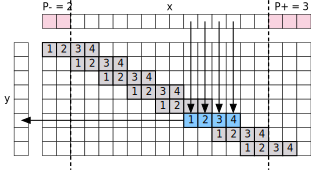
\includegraphics[width=0.7\textwidth]{figures/svg/conv}
	\caption{\textbf{Convolution.} The figure illustrates the process of filtering a 1D signal $\bx$ by a filter $f$ to obtain a signal $\by$. The filter has $H'=4$ elements and is applied with a stride of $S_h =2$ samples. The purple areas represented padding $P_-=2$ and $P_+=3$ which is zero-filled. Filters are applied in a sliding-window manner across the input signal. The samples of $\bx$ involved in the calculation of a sample of $\by$ are shown with arrow. Note that the rightmost sample of $\bx$  is never processed by any filter application due to the sampling step. While in this case the sample is in the padded region, this can happen also without padding.}\label{f:conv}
\end{figure}

The convolutional block is implemented by the function !vl_nnconv!. !y=vl_nnconv(x,f,b)! computes the convolution of the input map $\bx$ with a bank of $K$ multi-dimensional filters $\bff$ and biases $b$. Here
\[
 \bx\in\real^{H \times W \times D}, \quad
 \bff\in\real^{H' \times W' \times D \times D''}, \quad
 \by\in\real^{H'' \times W'' \times D''}.
\]
The process of convolving a signal is illustrated in \autoref{f:conv} for a 1D slice. Formally, the output is given by
\[
y_{i''j''d''}
=
b_{d''}
+
\sum_{i'=1}^{H'}
\sum_{j'=1}^{W'}
\sum_{d'=1}^D
f_{i'j'd} \times x_{i''+i'-1,j''+j'-1,d',d''}.
\]
The call !vl_nnconv(x,f,[])! does not use the biases. Note that the function works with arbitrarily sized inputs and filters (as opposed to, for example, square images). See \autoref{s:impl-convolution} for technical details.

\paragraph{Padding and stride.} !vl_nnconv! allows to specify  top-bottom-left-right paddings $(P_h^-,P_h^+,P_w^-,P_w^+)$ of the input array and subsampling strides $(S_h,S_w)$ of the output array:
\[
y_{i''j''d''}
=
b_{d''}
+
\sum_{i'=1}^{H'}
\sum_{j'=1}^{W'}
\sum_{d'=1}^D
f_{i'j'd} \times x_{S_h (i''-1)+i'-P_h^-, S_w(j''-1)+j' - P_w^-,d',d''}.
\]
In this expression, the array $\bx$ is implicitly extended with zeros as needed.

\paragraph{Output size.} !vl_nnconv! computes only the ``valid'' part of the convolution; i.e. it requires each application of a filter to be fully contained in the input support.  The size of the output is computed in \autoref{s:receptive-simple-filters} and is given by:
\[
  H'' = 1 + \left\lfloor \frac{H - H' + P_h^- + P_h^+}{S_h} \right\rfloor.
\]
Note that the padded input must be at least as large as the filters: $H +P_h^- + P_h^+ \geq H'$, otherwise an error is thrown.

\paragraph{Receptive field size and geometric transformations.} Very often it is useful to relate geometrically the indexes of the various array to the input data (usually images) in term of coordinate transformations and size of the receptive field (i.e. of the image region that affects an output). This is derived in \autoref{s:receptive-simple-filters}.

\paragraph{Fully connected layers.} In other libraries, a \emph{fully connected blocks or layers} are linear functions where each output dimension depends on all the input dimensions. \matconvnet does not distinguishes between fully connected layers and convolutional blocks. Instead, the former is a special case of the latter obtained when the output map $\by$ has dimensions $W''=H''=1$. Internally, !vl_nnconv! handle this case more efficiently when possible.

\paragraph{Filter groups.} For additional flexibility, !vl_nnconv! allows to group channels of the input array $\bx$ and apply to each group different subsets of filters. To use this feature, specify as input a bank  of $D''$ filters $\bff\in\real^{H'\times W'\times D'\times D''}$ such that $D'$ divides the number of input dimensions $D$. These are treated as $g=D/D'$ filter groups; the first group is applied to dimensions $d=1,\dots,D'$ of the input $\bx$; the second group to dimensions $d=D'+1,\dots,2D'$ and so on. Note that the output is still an array $\by\in\real^{H''\times W''\times D''}$.

An application of grouping is implementing the Krizhevsky and Hinton network~\cite{krizhevsky12imagenet} which uses two such streams. Another application is sum pooling; in the latter case, one can specify $D$ groups of $D'=1$ dimensional filters identical filters of value 1 (however, this is considerably slower than calling the dedicated pooling function as given in \autoref{s:pooling}).

% ------------------------------------------------------------------
\section{Convolution transpose (deconvolution)}\label{s:convt}
% ------------------------------------------------------------------

\begin{figure}[t]
	\centering
	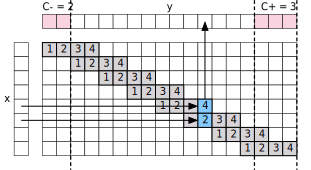
\includegraphics[width=0.7\textwidth]{figures/svg/convt}
	\caption{\textbf{Convolution transpose.} The figure illustrates the process of filtering a 1D signal $x$ by a filter $f$ to obtain a signal $y$. The filter is applied in a sliding-window, in a pattern that is the transpose of \autoref{f:conv}. The filter has $H'=4$ samples in total, although each filter application uses two of them (blue squares) in a circulant manner. The purple areas represented crops $C_-=2$ and $C_+=3$ which are discarded.  The samples of $x$ involved in the calculation of a sample of $y$ are shown with arrow. Note that, differently from \autoref{f:conv}, there is not any samples to the right of $\by$ which is not involved in a convolution operation. This is because the width $H''$ of the output $\by$, which given $H'$ can be determined up to $U_h$ samples, is selected to be the smallest possible.}\label{f:convt}
\end{figure}

The \emph{convolution transpose} block (sometimes referred to as ``deconvolution'') is the transpose of the convolution block described in \autoref{s:convolution}. In \matconvnet, convolution transpose is  implemented by the function !vl_nnconvt!. 

In order to understand convolution transpose, let:
\[
 \bx\in\real^{H \times W \times D}, \quad
 \bff\in\real^{H' \times W' \times D \times D''}, \quad
 \by\in\real^{H'' \times W'' \times D''}, \quad
\]
be the input tensor, filters, and output tensors. Imagine operating in the reverse direction by using the filter bank $\bff$ to convolve the output $\by$ to obtain the input $\bx$, using the definitions given in~\autoref{s:convolution} for the convolution operator; since convolution is linear, it can be expressed as a matrix $M$ such that  $\vv \bx = M \vv\by$; convolution transpose computes instead $\vv \by = M^\top \vv \bx$. This process is illustrated for a 1D slice in \autoref{f:convt}.

There are two important applications of convolution transpose The first one are the so called \emph{deconvolutional networks}~\cite{zeiler14visualizing} and other networks such as convolutional decoders that use the transpose of a convolution. The second one is implementing data interpolation. In fact, as the convolution block supports input padding and output downsampling, the convolution transpose block supports input upsampling and output cropping. 

Convolution transpose can be expressed in closed form in the following rather unwieldy expression (derived in \autoref{s:impl-convolution-transpose}):
\begin{multline}\label{e:convt}
y_{i''j''d''} = 
 \sum_{d'=1}^{D}
 \sum_{i'=0}^{q(H',S_h)}
 \sum_{j'=0}^{q(W',S_w)}
f_{
1+ S_hi' + m(i''+ P_h^-, S_h),\ %
1+ S_wj' + m(j''+ P_w^-, S_w),\ %
d'',
d'
} 
\times \\
x_{
1 - i' + q(i''+P_h^-,S_h),\ %
1 - j' + q(j''+P_w^-,S_w),\ %
d'
}
\end{multline}
where
\[
m(k,S) = (k - 1) \bmod S,
\qquad
q(k,n) = \left\lfloor \frac{k-1}{S} \right\rfloor,
\]
$(S_h,S_w)$ are the vertical and horizontal \emph{input upsampling factors},  $(P_h^-,P_h^+,P_h^-,P_h^+)$ the \emph{output crops}, and $\bx$ and $\bff$ are zero-padded as needed in the calculation. Note also that filter $k$ is stored as a slice $\bff_{:,:,k,:}$ of the 4D tensor $\bff$.

The height of the output array $\by$ is given by
\[
  H'' = S_h (H - 1) + H' -P^-_h - P^+_h.
\]
A similar formula holds true for the width. These formulas are derived in \autoref{s:receptive-convolution-transpose} along with expression for the receptive field of the operator.

We now illustrate the action of convolution transpose in an example (see also \autoref{f:convt}).  Consider a 1D slice in the vertical direction, assume that the crop parameters are zero, and that $S_h>1$. Consider the output sample $y_{i''}$ where the index $i''$ is chose such that $S_h$ divides $i''-1$; according to~\eqref{e:convt}, this sample is obtained as a weighted summation of $x_{i'' / S_h},x_{i''/S_h-1},...$ (note that the order is reversed). The weights are the filter elements $f_1$, $f_{S_h}$,$f_{2S_h},\dots$ subsampled with a step of $S_h$. Now consider computing the element $y_{i''+1}$; due to the rounding in the quotient operation $q(i'',S_h)$, this output sampled is obtained as a weighted combination of the same elements of the input $x$ that were used to compute $y_{i''}$; however, the filter weights are now shifted by one place to the right: $f_2$, $f_{S_h+1}$,$f_{2S_h+1}$, $\dots$. The same is true for $i''+2, i'' + 3,\dots$ until we hit $i'' + S_h$. Here the cycle restarts after shifting $\bx$ to the right by one place. Effectively, convolution transpose works as an \emph{interpolating filter}.

% ------------------------------------------------------------------
\section{Spatial pooling}\label{s:pooling}
% ------------------------------------------------------------------

!vl_nnpool! implements max and sum pooling. The \emph{max pooling} operator computes the maximum response of each feature channel in a $H' \times W'$ patch
\[
y_{i''j''d} = \max_{1\leq i' \leq H', 1 \leq j' \leq W'} x_{i''+i-1',j''+j'-1,d}.
\]
resulting in an output of size $\by\in\real^{H''\times W'' \times D}$, similar to the convolution operator of \autoref{s:convolution}. Sum-pooling computes the average of the values instead:
\[
y_{i''j''d} = \frac{1}{W'H'}
\sum_{1\leq i' \leq H', 1 \leq j' \leq W'} x_{i''+i'-1,j''+j'-1,d}.
\]
Detailed calculation of the derivatives are provided in \autoref{s:impl-pooling}.

\paragraph{Padding and stride.} Similar to the convolution operator of \autoref{s:convolution}, !vl_nnpool! supports padding the input; however, the effect is different from padding in the convolutional block as pooling regions straddling the image boundaries are cropped. For max pooling, this is equivalent to extending the input data with $-\infty$; for sum pooling, this is similar to padding with zeros, but the normalization factor at the boundaries is smaller to account for the smaller integration area.

% ------------------------------------------------------------------
\section{Activation functions}\label{s:activation}
% ------------------------------------------------------------------

\matconvnet supports the following activation functions:
%
\begin{itemize}
\item \emph{ReLU.} !vl_nnrelu! computes the \emph{Rectified Linear Unit} (ReLU):
\[
 y_{ijd} = \max\{0, x_{ijd}\}.
\]

\item \emph{Sigmoid.} !vl_nnsigmoid! computes the \emph{sigmoid}:
\[
 y_{ijd} = \sigma(x_{ijd}) = \frac{1}{1+e^{-x_{ijd}}}.
\]
\end{itemize}
%
See \autoref{s:impl-activation} for implementation details.

% ------------------------------------------------------------------
\section{Normalization}\label{s:normalization}
% ------------------------------------------------------------------

% ------------------------------------------------------------------
\subsection{Local response normalization (LRN)}\label{s:ccnormalization}
% ------------------------------------------------------------------

!vl_nnnormalize! implements a cross-channel normalization operator. Normalization applied independently at each spatial location and groups of channels to get:
\[
 y_{ijk} = x_{ijk} \left( \kappa + \alpha \sum_{t\in G(k)} x_{ijt}^2 \right)^{-\beta},
\]
where, for each output channel $k$, $G(k) \subset \{1, 2, \dots, D\}$ is a corresponding subset of input channels. Note that input $\bx$ and output $\by$ have the same dimensions. Note also that the operator is applied across feature channels in a convolutional manner at all spatial locations.

See \autoref{s:impl-ccnormalization} for implementation details.

% ------------------------------------------------------------------
\subsection{Batch normalization}\label{s:bnorm}
% ------------------------------------------------------------------

!vl_nnbnorm! implements batch normalization~\cite{ioffe2015}. Batch normalization is somewhat different from other neural network blocks in that it performs computation across images/feature maps in a batch (whereas most blocks process different images/feature maps individually). !y = vl_nnbnorm(x, w, b)! normalizes each channel of the feature map $\mathbf{x}$ averaging over spatial locations and batch instances. Let $T$ the batch size; then
\[
\mathbf{x}, \mathbf{y} \in \mathbb{R}^{H \times W \times K \times T},
\qquad\mathbf{w} \in \mathbb{R}^{K},
\qquad\mathbf{b} \in \mathbb{R}^{K}.
\]
Note that in this case the input and output arrays are explicitly treated as 4D tensors in order to work with a batch of feature maps. The tensors  $\mathbf{w}$ and $\mathbf{b}$ define component-wise multiplicative and additive constants. The output feature map is given by
\[
y_{ijkt} = w_k \frac{x_{ijkt} - \mu_{k}}{\sqrt{\sigma_k^2 + \epsilon}} + b_k,
\quad
\mu_{k} = \frac{1}{HWT}\sum_{i=1}^H \sum_{j=1}^W \sum_{t=1}^{T} x_{ijkt},
\quad
\sigma^2_{k} = \frac{1}{HWT}\sum_{i=1}^H \sum_{j=1}^W \sum_{t=1}^{T} (x_{ijkt} - \mu_{k})^2.
\]
See \autoref{s:impl-bnorm} for implementation details.

% ------------------------------------------------------------------
\subsection{Spatial normalization}\label{s:spnorm}
% ------------------------------------------------------------------

!vl_nnspnorm! implements spatial normalization. Spatial normalization operator acts on different feature channels independently and rescales each input feature by the energy of the features in a local neighborhood . First, the energy of the features is evaluated in a neighbourhood $W'\times H'$
\[
n_{i''j''d}^2 = \frac{1}{W'H'}
\sum_{1\leq i' \leq H', 1 \leq j' \leq W'} x^2_{
i''+i'-1-\lfloor \frac{H'-1}{2}\rfloor,
j''+j'-1-\lfloor \frac{W'-1}{2}\rfloor,
d}.
\]
In practice, the factor $1/W'H'$ is adjusted at the boundaries to account for the fact that neighbors must be cropped. Then this is used to normalize the input:
\[
y_{i''j''d} = \frac{1}{(1 + \alpha n_{i''j''d}^2)^\beta} x_{i''j''d}.
\]
See \autoref{s:spnorm} for implementation details.

% ------------------------------------------------------------------
\subsection{Softmax}\label{s:softmax}
% ------------------------------------------------------------------

!vl_nnsoftmax! computes the softmax operator:
\[
 y_{ijk} = \frac{e^{x_{ijk}}}{\sum_{t=1}^D e^{x_{ijt}}}.
\]
Note that the operator is applied across feature channels and in a convolutional manner at all spatial locations. Softmax can be seen as the combination of an activation function (exponential) and a normalization operator. See \autoref{s:impl-softmax} for implementation details.

% ------------------------------------------------------------------
\section{Losses and comparisons}\label{s:losses}
% ------------------------------------------------------------------

% ------------------------------------------------------------------
\subsection{Log-loss}\label{s:loss}
% ------------------------------------------------------------------

!vl_logloss! computes the \emph{logarithmic loss}
\[
 y = \ell(\bx,c) = - \sum_{ij} \log x_{ijc}
\]
where $c \in \{1,2,\dots,D\}$ is the ground-truth class. Note that the operator is applied across input channels in a convolutional manner, summing the loss computed at each spatial location into a single scalar.  See \autoref{s:impl-loss} for implementation details.

% ------------------------------------------------------------------
\subsection{Softmax log-loss}\label{s:sfloss}
% ------------------------------------------------------------------

!vl_softmaxloss! combines the softmax layer and the log-loss into one step for improved numerical stability. It computes
\[
y = - \sum_{ij} \left(
x_{ijc} - \log \sum_{d=1}^D e^{x_{ijd}}
\right)
\]
where $c$ is the ground-truth class. See \autoref{s:impl-sfloss} for implementation details.

% ------------------------------------------------------------------
\subsection{$p$-distance}\label{s:pdistance}
% ------------------------------------------------------------------

The !vl_nnpdist! function computes the $p$-th power $p$-distance between the vectors in the input data $\bx$ and a target $\bar\bx$:
\[
  y_{ij} = \left(\sum_d |x_{ijd} - \bar x_{ijd}|^p\right)^\frac{1}{p}
\]
Note that this operator is applied convolutionally, i.e. at each spatial location $ij$ one extracts and compares vectors $x_{ij:}$. By specifying the option !'noRoot', true! it is possible to compute a variant omitting the root:
\[
  y_{ij} = \sum_d |x_{ijd} - \bar x_{ijd}|^p, \qquad p > 0.
\]
See \autoref{s:impl-pdistance} for implementation details.

%% ------------------------------------------------------------------
%\subsection{Product}\label{s:product}
%% ------------------------------------------------------------------
%
%\[
% y_{ijd} = x^{(1)}_{ijd} x^{(2)}_{ijd}
%\]
%
%\paragraph{Implementation details.}
%\[
% \frac{dz}{dx^{(1)}_{ijd}}
%  =
% \sum_{i''j''d''}
%  \frac{dz}{dy_{i''j''d''}} 
%  \frac{dy_{i''j''d''}}{dx^{(1)}_{ijd}}
%  =
%  \frac{dz}{dy_{ijd''}} 
%  x^{(2)}_{ijd},
%  \qquad
%  \frac{dz}{dx^{(2)}_{ijd}}
%   =
%  \frac{dz}{dy_{ijd}} 
%  x^{(1)}_{ijd}.
%\]
%
%
%% ------------------------------------------------------------------
%\subsection{Split}\label{s:split}
%% ------------------------------------------------------------------
%
%\[
% y_{ijd}^{(1)} = x_{ijd}, \qquad y_{ijd}^{(2)} = x_{ijd}
%\]
%
%\[
% \frac{dz}{dx_{ijd}} =
%\sum_{i''j''d''} 
% \frac{dz}{dy_{i''j''d''}^{(1)}}
%  \frac{dy_{i''j''d''}^{(1)}}{dx_{ijd}}
% +
%  \frac{dz}{dy_{i''j''d''}^{(2)}}
%  \frac{dy_{i''j''d''}^{(2)}}{dx_{ijd}}
%\]
